\lhead[\thepage]{CHAPTER \thechapter. STATE OF THE ART}
\chead[]{}
\rhead[WepSIM: Simulador de procesador elemental con unidad de control microprogramada\leftmark]{\thepage}
\renewcommand{\headrulewidth}{0.5pt}

\lfoot[]{}
\cfoot[]{}
\rfoot[]{}
\renewcommand{\footrulewidth}{0pt}

%% This is an example first chapter.  You should put chapter/appendix that you
%% write into a separate file, and add a line \include{yourfilename} to
%% main.tex, where `yourfilename.tex' is the name of the chapter/appendix file.
%% You can process specific files by typing their names in at the 
%% \files=
%% prompt when you run the file main.tex through LaTeX.
\chapter{Estado del arte}
\label{ch:state_of_the_art}
\markboth{}{STATE OF THE ART}

Este capítulo presenta el estado del arte, la última y más avanzada etapa de las tecnologías relacionadas con nuestra aplicación. Primero, se presentan los diferentes simuladores existentes para microprogramación (Section \ref{sec:simuladores_microprogramacion}). Después, se presentan los diferentes simuladores existentes para la programación en código ensamblador (Section \ref{sec:simuladores_ensamblador}). Por último, realizamos una comparación de nuestro trabajo con el contexto actual de los distintos simuladores expuestos previamente (Section \ref{sec:propuesta_simulacion}).

\section{Simuladores para microprogramación}
\label{sec:simuladores_microprogramacion}

En esta sección, se explican los diferentes simuladores existentes para la microprogramación. Cabe destacar, que actualmente existen pocos simuladores que nos proporcionen esta funcionalidad, debido a que una gran parte de ellos, son utilizados de forma interna por las empresas para verificar el correcto funcionamiento de sus unidades en la fase de diseño y desarrollo. En primer lugar, vamos a centrarnos en los simuladores que están más enfocados a una labor docente.

En \cite{yen1986development}, se describe el desarrollo y la implementación de un simulador para una arquitectura de microprogramación específica. Fue publicado en el año 1986, y estaba basado en la arquitectura definida  



\section{Simuladores para programación en ensamblador}
\label{sec:simuladores_ensamblador}
En esta sección, se explican los diferentes simuladores existentes para la programación en ensamblador. Los simuladores más conocidos para labores docentes, son SPIM, MARS y WebMIPS.

SPIM \cite{larus1990spim}, es un simulador de un procesador MIPS de 32 bits desarrollado a principios de 1990. En un primer momento implementaba el juego de instrucciones MIPS-1, utilizado por los computadores MIPS R2000/R3000. Actualmente, implementa la arquitectura MIPS32 más reciente y sus instrucciones adicionales. Permite ejecutar programas en ensamblador para esta arquitectura. Además, también permite depurar el código implementado, de forma que el alumno pueda corregir con mayor facilidad los errores cometidos. Este simulador, fue creado por James R. Larus y tiene versiones compiladas para Windows, Mac OS X y Unix/Linux e incluso tiene una versión básica para Android, aunque su diseño no está pensado para dispositivos móviles. Puesto que el simulador está totalmente enfocado al procesador MIPS, posee el juego completo de instrucciones para la versión de 32 bits del procesador y todas las directivas de las que consta el lenguaje. Otra característica que hace de SPIM un potente simulador, es proveer de un pequeño sistema operativo que soporta las principales llamadas al sistema mediante la instrucción syscall. SPIM, es un simulador que permite múltiples configuraciones mediante su interfaz de usuario, de manera que se puede indicar:

\begin{itemize}

\item Activación del uso de pseudoinstrucciones.

\item Simulación de predicción de saltos y accesos a memoria, con la latencia correspondiente.

\item Activación del uso del manejador de la señal trap y la carga del manejador personalizado.

\item Activación de la visualización de los mensajes en caso de ocurrir excepciones.

\item Activación del uso de "memory-mapped IO".

\end{itemize}

\begin{figure}[htbp]
 	\centering
 	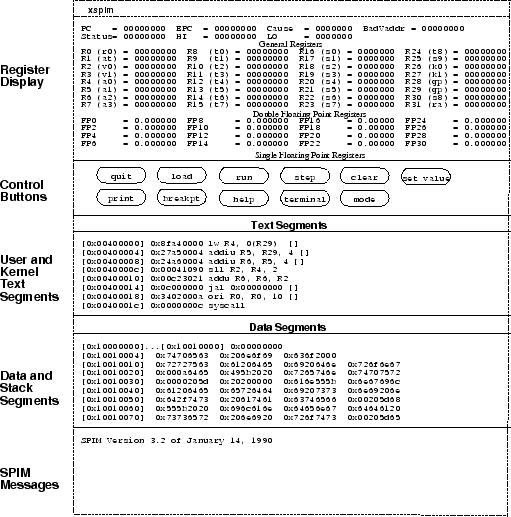
\includegraphics[width=8cm]{figures/spim_figure}
 	\caption{Interfaz SPIM.}
	\label{fig:spim_figure}
\end{figure}

SPIM, además cuenta con una versión más actualizada del simulador, que posee una interfaz gráfica más potente. Éste simulador se llama QtSPIM \cite{aguilar2013simuladores}, y cuenta con todas las características anteriormente mencionadas de SPIM.

\begin{figure}[htbp]
 	\centering
 	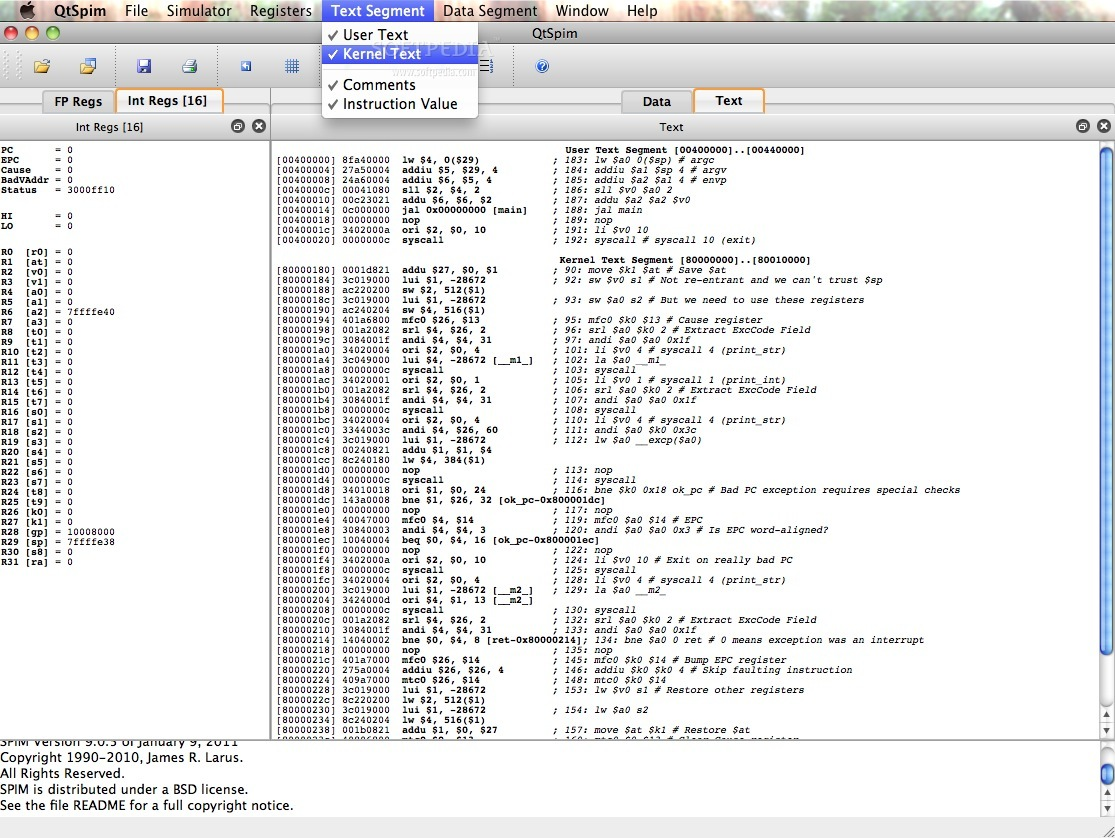
\includegraphics[width=12cm]{figures/qtspim_figure}
 	\caption{Interfaz QtSPIM.}
	\label{fig:qtspim_figure}
\end{figure}

MARS \cite{vollmar2006mars}, es un simulador con interfaz gráfica desarrollado en JAVA para el lenguaje ensamblador MIPS. Fue creado en el año 2005 como una alternativa del simulador SPIM y diseñado específicamente para las necesidades limitadas de cusos de pregrado. Está basado en la arquitectura MIPS RISC, que tiene un número pequeño de elementos del lenguaje e instrucciones. Consta de operaciones de entrada/salida, saltos, condiciones y operaciones aritmético-lógicas tanto enteras como en coma flotante. Alguna de las mejoras que incorpora MARS con respecto a SPIM son \cite{vegdahl2008mipspilot}: 

\begin{itemize}

\item Depuración más sencilla y cómoda, debido constar de GUI. Ésto se debe, a que para añadir un punto de ruptura, únicamente hay que clickar sobre un checkbox que tiene la instrucción.

\item Los programas puedes ejecutarse de forma inversa, lo que permite volver a un estado anterior de la máquina en la ejecución de un programa.

\item La velocidad de ejecución puede modificarse, de forma que si se ralentiza el usuario puede observar como cada instrucción se resalta cuando está siendo ejecutada y ver los cambios que se producen en los valores del banco de registros y de las ubicaciones de memoria.

\item  La memoria y los registros se pueden modificar de una manera WYSIWYG.

\item Incorpora un editor de texto, eliminando dependencias externas para el uso del simulador.

\item Permite que los desarrolladores puedan suministrar nuevos complementos, que por ejemplo, sirvan para extender la arquitectura o mostrar los datos de forma intuitiva.

\end{itemize}

\begin{figure}[htbp]
 	\centering
 	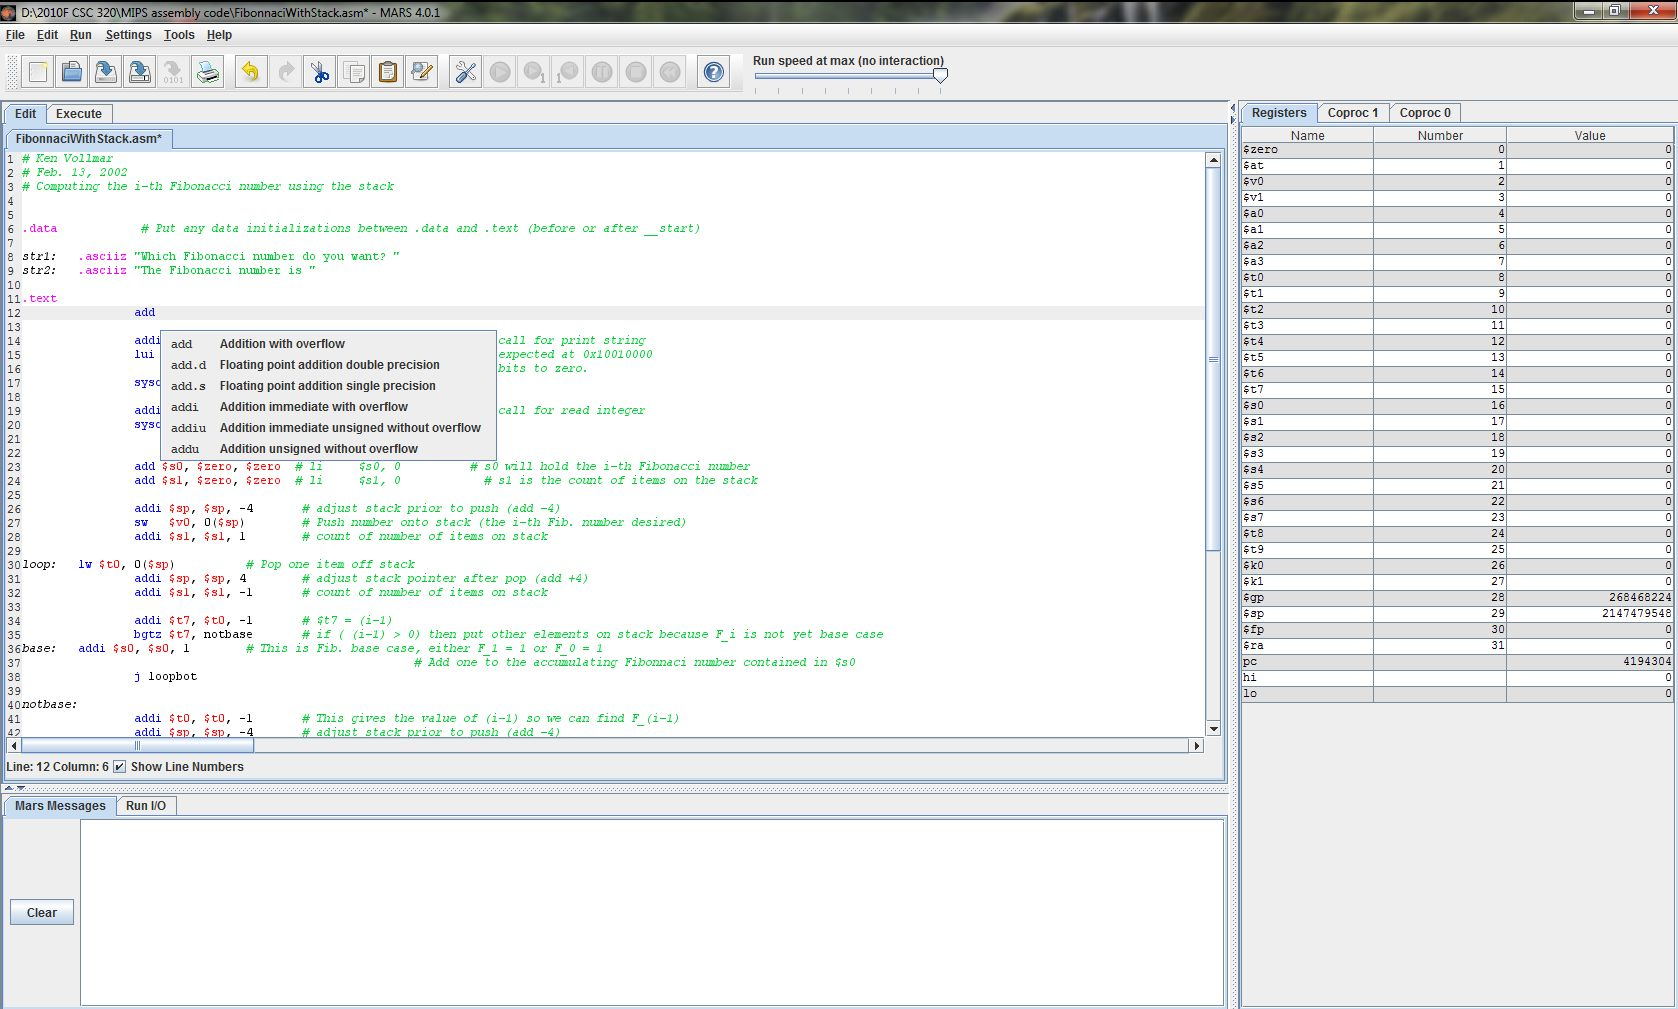
\includegraphics[width=12cm]{figures/mars_figure}
 	\caption{Interfaz MARS.}
	\label{fig:qtspim_figure}
\end{figure}

em88110, es emulador descrito en \cite{perez1997em88110} que se basa en la emulación de un procesador superescalar. El propósito fundamental de este emulador, es mostrar el funcionamiento de este tipo de procesadores, haciendo visible el funcionamiento del pipeline y las dependencias existentes. Está basado en una arquitectura específica (MC88110) y pese a integrar el efecto de un procesador superescalar no integra la microprogramación, que haría de él un emulador completo.

\begin{figure}[htbp]
 	\centering
 	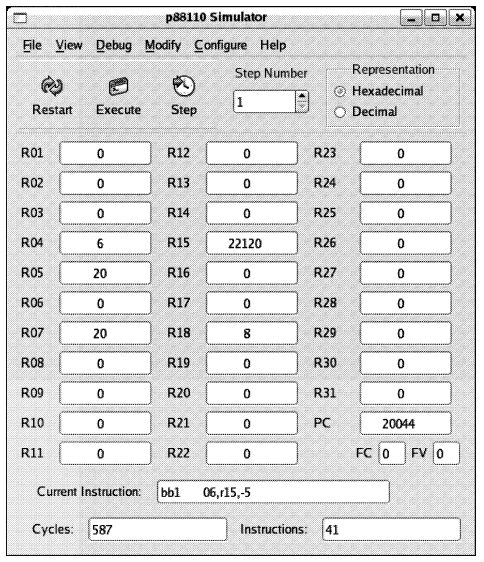
\includegraphics[width=12cm]{figures/em88110}
 	\caption{Interfaz em88110.}
	\label{fig:em88110_figure}
\end{figure}


WebMIPS \cite{branovic2004webmips}, es un simulador desarrollado en la Facultad de Ingeniería de la Información de Sienna, Italia. Está escrito en el lenguaje de programación ASP.NET y se utiliza mediante una página web, de forma que no requiere de su instalación en local. No soporta el juego completo de instrucciones de MIPS, sino que consta de un juego reducido de instrucciones que sirve de intruducción al estudio de arquitectura de computador. Con respecto a los anteriores simuladores mencionados, difiere al mostrar el esquema arquitectónico, indicando las 5 etapas de pipeline de las que consta el computador que simula. Otra característica, es la indicación del número de ciclos de reloj que consume la ejecución del programa. Tiene como objetivo principal la demostración de la ejecución del juego de instrucciones básico explicado durante la asignatura "Arquitectura de Computadores" impartida por los creadores del simulador.

Entre las diferentes características a destacar de este simulador, se encuentran:

\begin{itemize}
	
\item Verificación del código ensamblador, comprobando que no existen errores en la definición el código.

\item Dispone de códigos simples de ejemplo ("load-and-play") que facilitan la comprensión del funcionamiento del procesador.

\item Permite diferentes visualizaciones del estado de la memoria y los registros del procesador.

\item Consta de dos modos de ejecución: paso a paso y ejecución completa del programa.
	
\end{itemize}

\begin{figure}[htbp]
 	\centering
 	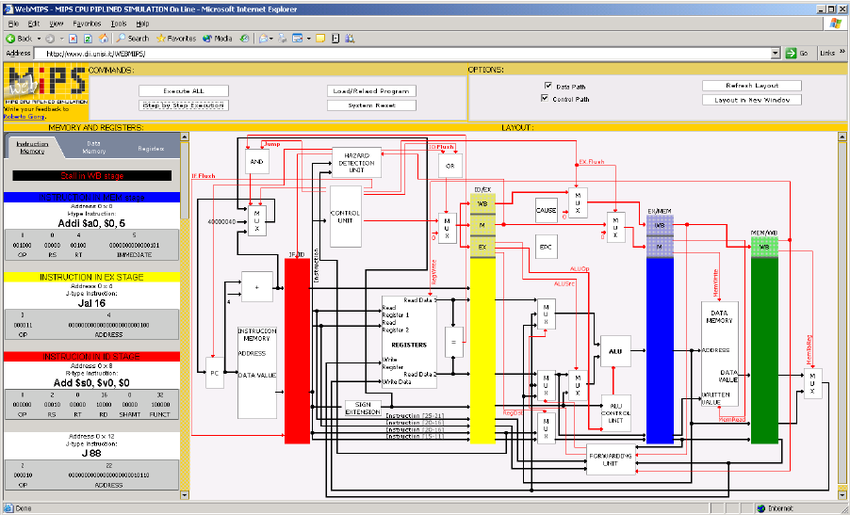
\includegraphics[width=12cm]{figures/webmips_figure}
 	\caption{ Interfaz WebMIPS.}
	\label{fig:qtspim_figure}
\end{figure}

\clearpage

\section{Propuesta de simulación unificada}
\label{sec:propuesta_simulacion}
Hay distintas herramientas muy útiles para labores docentes relacionadas con la asignatura Estructura de Computadores, aunque como se comento previamente, no existe una herramienta que nos proporcione el desarrollo y simulación tanto a nivel de microcódigo como a nivel de ensamblador. WepSIM, une ambos aspectos ofreciendo:

\begin{itemize}
	\item Visión interrelacionada de la microprogramación y la programación en ensamblador.
	\item Flexibilidad en la plataforma usada, pensando el dispositivos móviles.
	\item Herramienta autocontenida, de forma que incorpora en sí misma tanto la ayuda como distintos ejemplos que favorecen la comprensión del simulador.
	\item Consta de un modelo hardware que puede ser modificado o ampliado en caso de ser necesario.
	\item Permite definir un amplio conjunto de instrucciones máquina.
	\item Puede ser usado como herramienta de microprogramación o de programación en ensamblador.
\end{itemize}

De este modo, con WepSIM se pretende crear un simulador unificado, abarcando los aspectos más relevantes de la asignatura "Estructura de Computadores" y permitiendo que todas las prácticas de la asignatura puedan realizarse en la misma plataforma, evitando la pérdida de tiempo y dificultad que supone para el alumno el habituarse a diferentes entornos para cada una de las prácticas.

WepSIM, se puede definir por tanto como un simulador de programación en ensamblador y microprogramación, flexible puesto que permite la personalización del juego de instrucciones de la máquina, multiplataforma puesto que permite su uso desde diferentes tipos de dispositivos, e interactivo al poder modificar la configuración de la máquina en tiempo de ejecución.

\begin{table}[htbp]
\ra{1.2}
\centering
%\resizebox{\textwidth}{%
\resizebox{\textwidth}{!}{
\begin{tabular}{@{}llllllll@{}}
\toprule
Simulador & SPIM & MARS & PC88110 & WebMIPS & WepSIM  & P8080E & MicMac\\ 
\midrule
Ensamblador				& \ding{51} & \ding{51} & \ding{51} & \ding{51} & \ding{51} &  &  \\
\midrule
Microprogramación				&  &  &  &  & \ding{51} & \ding{51} & \ding{51} \\
\midrule
Multiplataforma				& \ding{51} &  &  & \ding{51} & \ding{51} &  &  \\
\midrule
Interactivo				&  &  &  &  & \ding{51} &  &  \\
\midrule
Juego de instrucciones personalizable				&  &  &  &  & \ding{51} &  &  \\
\bottomrule
\end{tabular}
}
\caption{Comparación de simuladores de ensamblador y microcódigo.}
\label{tab:comparison_frameworks}
\end{table}

